%\chapter{Preliminares. } % (fold)
\chapter{Marco Teórico}
El contenido de este capítulo abordará temas estrechamente relacionados con la criptograf\'ia. Se abordará información acerca de los 2 tipos de criptografía que existen, criptograf\'ia sim\'etrica y asim\'etrica. En el caso de la criptograf\'ia sim\'etrica se describir\'an dos primitivas criptogr\'aficas, los cifradores por bloque y las funciones hash. 
Respecto a la criptograf\'ia asim\'etrica o de clave p\'ublica, se hablar\'a sobre el algoritmo de cifrado RSA, firmas digitales y firmas a ciegas, todas \'estas primitivas juegan un papel fundamental para el funcionamiento de este proyecto. De igual forma se describe con detalle los servicios que ofrece el cómputo nube, haciendo énfasis en un servicio en particular que es el almacenamiento que se utilizará para la implementación de este protocolo criptográfico. 
%Un tópico de gran importancia dentro de este protocolo son las funciones hash criptográficas, dichas funciones son mencionadas en este capítulo, al igual que las firmas digitales, firmas a ciegas y firmas digitales con RSA ya que estas j. 







\section{Criptografía. }

La \textit{ criptografía } tiene como objetivo fundamental habilitar a dos personas usualmente referidas como Alice y Bob para que se comuniquen sobre un canal inseguro de tal manera que un adversario, Oscar, no pueda entender que es lo que están diciendo, éste canal podría ser una línea telefónica o una red de computadora, por ejemplo. La información que quiere enviar Alice a Bob que nosotros llamaremos “texto en claro”, puede ser un texto en inglés, datos numéricos, o cualquier cosa---esta estructura es completamente arbitraria. Alice cifra el texto en claro usando una llave predeterminada y envía el texto cifrado resultante sobre el canal. Oscar, al ver el texto cifrado en el canal que está escuchando a escondidas, no puede determinar qué es el texto en claro; pero Bob, quien sabe la llave con la que se cifró el archivo, puede descifrar el texto y obtener el texto claro ~\cite{stinson}.\\

Esta ciencia que mantiene la información segura se encuentra dividida en dos tipos: \textit{Criptografía Simétrica} y \textit{Criptografía Asimétrica}. La \textit{ criptografía simétrica} o también llamada criptografía de llave secreta, basa su seguridad en una sola llave que se comparte entre dos entidades que quieren compartir información, dicha llave es utilizada para cifrar un archivo al ser enviado a la otra entidad y este utilizará la misma llave para descifrarlo cuando lo reciba. El esquema de cifrado simétrico se puede representar a través de la siguiente figura ~\ref{fig:2-3-1}. \\

\begin{figure}[H]
\centering
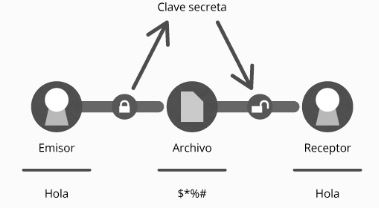
\includegraphics[width=10cm, height=5cm]{./images/Cripto_Simetrica.JPG}
\caption{Diagrama de Criptografía Simétrica.}
\label{fig:2-3-1}
\end{figure}

Los algoritmos criptográficos simétricos tienen dos versiones: cifrador en bloque y cifrador de flujo. El beneficio en cuanto al uso de un algoritmo simétrico se encuentra en el procesamiento rápido para cifrar y descifrar un alto volúmen de datos. El cifrado simétrico es una práctica eficaz de almacenamiento de información sensible en una base de datos, un registro o archivo ~\cite{sime}. \\

La \textit{ criptografía asimétrica} o criptografía de llave pública involucra el uso de un par de llaves para cada entidad que desea comunicarse, estas llaves llamadas pública y privada. Para que una entidad envíe un archivo a otra, necesita cifrar el archivo con la llave pública de esa entidad a la que se desea enviar, y cuando lo reciba esa entidad lo deberá descifrar con su llave privada o secreta. De esta manera se evita el compartir llaves para cifrar y descifrar como sucede en la criptografía simétrica y reduce los riesgos de un ataque de adversarios. El cifrado asimétrico puede ser representado como aparece en la figura ~\ref{fig:2-4-1}. \\

\begin{figure}[H]
\centering
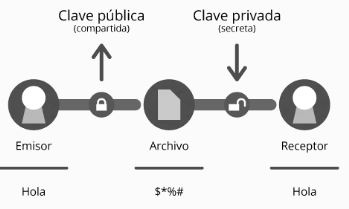
\includegraphics[width=10cm, height=5cm]{./images/Cripto_Asimetrica.JPG}
\caption{Diagrama de Criptografía Asimétrica.}
\label{fig:2-4-1}
\end{figure}

Los beneficios de la criptografía asimétrica son que las claves públicas pueden ser distribuidas con toda tranquilidad, pues no puedes hacer uso de las llaves públicas sin las llaves privadas. Asimismo, el cifrado asimétrico se emplea frecuentemente para elaborar firmas digitales, un mecanismo que permite al receptor de un mensaje firmado digitalmente poder identificar a la entidad que origino ese mensaje y de esa manera confirmar que el mensaje no ha sido alterado. \\



%==================================================================================================================================================================
Los servicios criptográficos son aquellos que garantizan en un sistema de información la adquisición, almacenamiento, procesamiento y transmisión de la información y para lograrlo se valen de uno o más objetivos fundamentales. 
\begin{itemize}
\item \textbf{Confidencialidad. }
Es un servicio utilizado para garantizar que solo las personas autorizadas tienen acceso a la información.
%mantener el contenido de la información de todos, excepto los autorizados a tenerla. El secreto es un término sinónimo de confidencialidad y privacidad.
%Hay numerosos enfoques para proporcionar confidencialidad, que van desde la protección física a los algoritmos matemáticos que hacen que los datos sean ininteligibles.

\item \textbf{Autenticación. }
Esta función se aplica tanto a las entidades como a la propia información. Dos entidades que participan en una comunicación deben identificarse entre sí. La información entregada a través de un canal debe ser autenticada en cuanto al origen, fecha de origen, contenido de los datos, tiempo enviado, etc. 

\item \textbf{Integridad. }
Es un servicio que se ocupa de la alteración no autorizada de los datos. Para asegurar la integridad de los datos, se debe tener la capacidad de detectar la manipulación de datos por parte de algún adversario. La manipulación de datos incluye inserción, supresión y sustitución, entre otros.

\item \textbf{No repudio. }
Es un servicio que impide a una entidad negar compromisos o acciones anteriores. Cuando surgen disputas debido a que una entidad niega que se tomaron ciertas acciones, es necesario un medio para resolver la situación. Por ejemplo, una entidad puede autorizar la compra de una propiedad por otra entidad y posteriormente negar que se concedió dicha autorización ~\cite{menezes}.
\end{itemize}


El \textit{ Criptoanálisis } es la ciencia que se ocupa del análisis de un texto cifrado para obtener la información original sin conocimiento de la clave secreta, esto es, de forma ilícita rompiendo así los procedimientos de cifrado establecidos por la Criptografía, por lo que se dice que Criptoanálisis y Criptografía son ciencias complementarias pero contrarias ~\cite{cripto}. \\


Los \textit{ataques a servicios criptográficos } son una violación a la seguridad de la información realizada por intrusos que tienen acceso físico al sistema sin ningún tipo de restricción, su objetivo es robar la información o hacer que ésta pierda valor relativo, o que disminuyan las posibilidades de su supervivencia a largo plazo.\\
\begin{itemize}
\item Ataque sólo con texto cifrado. Este caso es cuando el criptoanalísta sólo conoce el criptograma y el algoritmo con que fue generado; con esta información pretende obtener el texto en claro.
\item Ataque con texto en claro conocido. En esta situación el criptoanalísta conoce mensajes en claro seleccionados por él mismo y sus correspondientes criptogramas, así como el algoritmo con que éstos fueron generados; aquí el objetivo es conocer la clave
secreta y poder descifrar libremente cualquier texto. 
\item Ataque con texto cifrado escogido. El criptoanalísta conoce el algoritmo de cifrado, así como un criptograma seleccionado por él mismo y su correspondiente texto en claro, su objetivo es obtener el mensaje en claro de todo criptograma que intercepte.
\item Ataque con texto en claro escogido. En este caso el criptoanalísta además de conocer el algoritmo de cifrado y el criptograma que quiere descifrar, también conoce el criptograma de un texto en claro ~\cite{ataques}.
\end{itemize} 

%==================================================================================================================================================================
\section{Cifrador por bloques. }

Un cifrador de bloques es una función que convierte bloques de texto de \textit{n} bits a bloques de texto cifrado de \textit{n} bits; a \textit{n} se denomina longitud de bloque. La función que convierte los bloques de texto simple está parametrizada por una clave \textit{K} de \textit{ k}-bits , tomando valores de un subconjunto $\cal{K}$ (el espacio de la llave) del conjunto de todas las palabras numéricas de \textit{$ \{ 0,1 \} ^{k}$}. Generalmente la clave \textit{K} se elige al azar. El uso de bloques de texto claro y texto cifrado de igual tamaño evita la expansión de datos ~\cite{menezes}. \\

Para los bloques de texto de \textit{n}-bit, texto cifrado de \textit{n}-bit y una clave fija de \textit{n}-bit, la función de cifrado es
una biyección, es decir que el texto cifrado debe ser siempre diferente pero cuando se descifre este debe corresponder al texto en claro, definiendo una permutación de palabras numéricas de \textit{n}-bits. Cada clave potencial define una biyección diferente. El número de llaves es de longitud | $\cal{K}$ |, y el tamaño efectivo de la clave es de longitud | $\cal{K}$ |. Esto es igual a la longitud de la clave si todos las palabras numéricas de \textit{k}-bits son claves válidas ($\cal{K}$ = $V_{\textit{k}}$). Si las llaves son equiprobables (misma probabilidad) y cada una define una biyección diferente, la entropía (medida de incertidumbre) del espacio clave es también de longitud | $\cal K$ | ~\cite{menezes}. \\ \\


Los cifradores por bloques más usados son AES \textit{(Advanced Encryption Standard}, por sus 
siglas en ingl\'es) y \textit{DES (Data Encryption Standard, por sus siglas en inglés)} ~\cite{bloques}.\\ 

Los cifradores por bloques pueden ser representados como se ve en la figura ~\ref{fig:2-5-1}.

\begin{figure}[H]
\centering
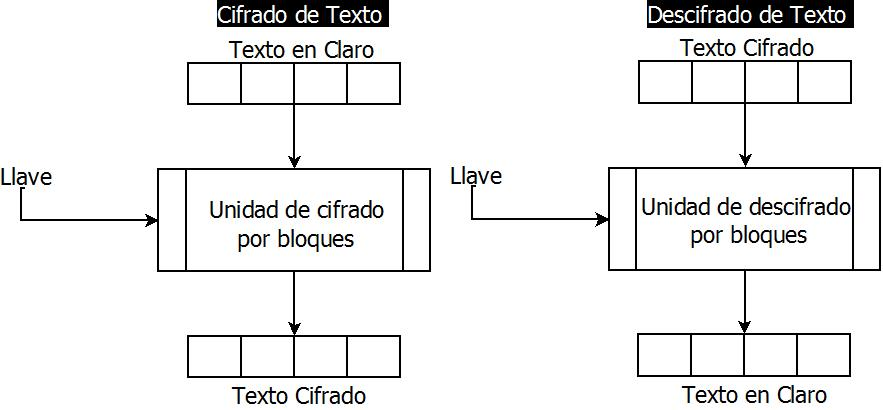
\includegraphics[width=10cm, height=5cm]{./images/CifradoBloques.jpeg}
\caption{Diagrama de Cifradores por Bloques}
\label{fig:2-5-1}
\end{figure}

%==================================================================================================================================================================

\section{Funciones Hash. }
A continuación, se describirán las características de las {\it funciones hash}, también conocidas como {\it funciones de resumen}. Las funciones hash basan su definición en funciones de un solo sentido ({\it one-way functions}, en inglés). Una función de un solo sentido es aquella que para un valor $x$, es muy fácil calcular $f(x)$, pero es muy difícil hallar $f^{-1}(x)$. Es complicado en general, hallar funciones de este tipo y probar que lo son.
\begin{definition}
Una función hash, es una función de un solo sentido cuya entrada $m$ es un mensaje de longitud arbitraria y la salida es una cadena binaria de longitud fija. Al resumen o hash de un mensaje $m$, se le denotará como $h(m)$. Una propiedad de las funciones hash es que sea imposible que se produzca una colisión ya sea débil o fuerte, además de resistir ataques de pre imagen.
%\begin{itemize}
% \item Para cualquier mensaje $m$, debe ser posible calcular $h(m)$ eficientemente. 
% \item Dado $h(m)$, debe ser computacionalmente difícil, hallar un mensaje $m'$, tal que $h(m)=h(m')$.
% \item Debe ser computacionalmente difícil, hallar dos mensajes $m$ y $m'$ tales que $h(m)=h(m')$.
%\end{itemize}
\end{definition}
Entre las funciones hash que se usan para criptograf\'ia est\'an: MD2, MD4, MD5, donde MD significa {\it Message Digest}, y el algoritmo est\'andar al momento de escribir \'estas notas es el {\it Secure Hash Algorithm} por sus siglas en ingl\'es SHA.
La MD5 fue dise\~nada por Ron Rivest, toma como entrada un mensaje de longitud arbitraria y proporciona como salida una cadena binaria de 128 bits.

Dentro de SHA-2 encontramos varios tipos, el SHA-224, SHA-256, SHA-384 y SHA-512. El más seguro, es el que da mayor salida de bits que es el SHA-512, con una salida de 512 bits, que tiene 80 rondas (pasos).
En la SHA-256, tenemos una longitud de palabra de 323 bits, con 64 rondas, tamaño del bloque de 512 bits, y con una salida de 256 bits.
Como ocurre con todos los cifrados y hash, cuanto más seguro, más lento su procesamiento y uso, debemos encontrar un equilibrio entre seguridad y velocidad.

%La SHA 256 fue dise\~nada por el NIST y se estableci\'o como est\'andar en 1993. Recibe como entrada un mensaje con longitud menor a $2^{64}$ bits y
%como salida se obtiene una cadena binaria de 160 bits. Al igual que el MD5, se procesa en bloques de 512 bits ~\cite{modes}.


%==================================================================================================================================================================


\section{RSA}

El esquema de criptografía RSA se llama así por los nombres de los autores Ron Rivest, Adi Shamir y Leonard Adleman, es actualmente el esquema criptográfico asimétrico más utilizado. RSA fue patentado en los Estados Unidos (pero no en el resto del mundo) hasta el 2000. Utiliza una clave pública, la cual se distribuye (en forma autenticada preferentemente), y otra privada, la cual es guardada en secreto por su propietario. Cuando se envía un mensaje, el emisor busca la clave pública de cifrado del receptor y una vez que dicho mensaje llega al receptor, éste se ocupa de descifrarlo usando su clave oculta. Los mensajes enviados usando el algoritmo RSA se representan mediante números y el funcionamiento se basa en el producto de dos números primos grandes (mayores que 10100) elegidos al azar para conformar la clave de descifrado. Emplea expresiones exponenciales en aritmética modular. La seguridad de este algoritmo radica en que no hay maneras rápidas conocidas de factorizar un número grande en sus factores primos utilizando computadoras tradicionales.
La computación cuántica podría proveer una solución a este problema de factorización. Este popular sistema se basa en el problema matemático de la factorización de números grandes. \\
El algoritmo RSA funciona de la siguiente manera: \\

\textbf{Generación de llaves.} Estos son los pasos involucrados en el cálculo de la clave pública y privada para un criptosistema
RSA. \\
\begin{itemize}
\item Inicialmente es necesario generar aleatoriamente dos números primos grandes, a los que llamaremos \textit{p} y \textit{q}.
\item A continuación calcularemos \textit{n} como producto de \textit{p} y \textit{q: n = p * q}
\item Se calcula \textit{$ \phi : \phi (n)=(p-1)(q-1)$}
\item Se elige al azar un entero $e$, tal que $mcd(e, \phi(n))=1$, es decir $e$ es 
primo relativo con $\phi(n)$. 
%\item Se calcula un número natural $e$ de manera que $mcd(e, \fi(n))=1$ , es decir $e$ debe ser primo relativo de $\phi(n)$. 
\item Se calcula $d$ tal que $ed \bmod \phi (n)=1$. 
\item El par de números \textit{(e,n)} son la clave pública.
\item El par de números \textit{(d,n)} son la clave privada.
\end{itemize} 
\textbf{Cifrado y descifrado.}
Despu\'es de que un usuario tenga su par de llaves, ser\'a posible realizar las operaciones para cifrar y descifrar como se muestra a continuaci\'on
% El cifrado y descifrado RSA se realiza en el campo de los numeros enteros \textit{Zn} y los cálculos modulares desempeñan un papel central. RSA cifra el texto en claro \textit{x}, donde consideramos que la cadena de bits que representa \textit{x} es un elemento en \textit{Zn = 0,1, ..., n-1} . Como consecuencia, el valor binario del texto en claro \textit{x} debe ser menor que \textit{n}. Lo mismo ocurre con el texto cifrado. El cifrado con la clave pública y el descifrado con la clave privada son los siguientes:


\begin{itemize}
\item Cifrado: la función de cifrado es $C = M^e \bmod n$.

\item Descifrado: la función de descifrado es $M = C^d \bmod n$.
\end{itemize} 
\noindent
{\bf Ejemplo.} El primer paso es calcular las llaves p\'ublica y privada. Si se consideran los primos $p = 11$ y $q = 23$ entonces $n = 11 * 23 = 253$ y $ \phi = ( 11 - 1 ) * ( 23 - 1 ) = 220 $.
\noindent
Si se escoge $e=3$, es f\'acil verificar que $mcd ( 220, 3 ) = 1$. En tanto que $d=147$ 
que $3 * 147 \bmod 220 =1$. Por lo tanto, la clave p\'ublica ser\'a $(e,n) = (3,253)$ y 
la clave privada $(d,n) = (147,253)$.\\ 
%donde: \textit{( 11 - 1 ) = 10} y \textit{( 22 - 1 ) = 22 }\\

%\textit{e = 3} \\
%
%\textit{MCD ( 220, 3 ) = 1} \\
%
%\textit{d = inv (3, 220) = 147 } \\


%Clave pública: \textit{ } \\
%
%Clave privada: \textit { (d,n) = (147,253) } \\
\noindent

\textbf{ Cifrado: }\\

Cifraremos la palabra seguridad y para esto le asignaremos números a todas las letras del abecedario dando como resultado para nuestra palabra los siguientes valores: \\

\begin{tabular}{ |p{1cm}|p{1cm}|p{1cm}|p{1cm}|p{1cm}|p{1cm}|p{1cm}|p{1cm}|p{1cm}| }
\hline
{ S } & { E } & { G } & { U } & { R } & { I } & { D } & { A } & { D } \\
\hline
{ 18 } & { 4 } & { 6 } & { 20 } & { 17 } & { 8 } & { 3 } & { 0 } & { 3 } \\
\hline
\end{tabular}
\\ \\

Tenemos el mensaje \textit{ M = 18 4 6 20 17 8 3 0 3 } a cifrar\\

\textit{$ 18^{3} = 5832 \mod 253 = 13$} \\

\textit{$ 4^{3} = 64 \mod 253 = 64$} \\

\textit{$ 6^{3} = 216 \mod 253 = 216 $} \\ 

\textit{$ 20^{3} = 8000 \mod 253 = 157 $} \\

\textit{$ 17^{3} = 4913 \mod 253 = 106 $}\\

\textit{$ 8^{3} = 512 \mod 253 = 6 $}\\

\textit{$ 3^{3} = 27 \mod 253 = 27 $}\\

\textit{$ 0^{3} = 0 \mod 253 = 0 $}\\

\textit{$ 3^{3} = 27 \mod 253 = 27 $}\\

Obtenemos el mensaje cifrado \textit{ C = 13 64 216 157 106 6 27 0 27} \\

\textbf{Descifrado: } \\

Tenemos el texto cifrado, \textit{ C = 13 64 216 157 106 6 27 0 27} \\

\textit{$ 13^{147} \mod 253 = 18$} \\

\textit{$ 64^{147} \mod 253 = 4$} \\

\textit{$ 216^{147} \mod 253 = 6$} \\

\textit{$ 157^{147} \mod 253 = 20$} \\

\textit{$ 106^{147} \mod 253 = 17$} \\

\textit{$ 6^{147} \mod 253 = 8$} \\

\textit{$ 27^{147} \mod 253 = 3$} \\

\textit{$ 0^{147} \mod 253 = 0$} \\

\textit{$ 27^{147} \mod 253 = 3$} \\

Obtenemos el mensaje descifrado, \textit{ M = 18 4 6 20 17 8 3 0 3} \\

% https://cs.uns.edu.ar/~ldm/mypage/data/ss/info/ejemplo-rsa.pdf

%==================================================================================================================================================================

\section{Firma digital}

Una \textit{firma digital} es un mecanismo de autenticación que permite al creador de un mensaje fijar un código que actúa como una firma. La firma es formada tomando el hash del mensaje y cifrar el mensaje con clave privada del creador. La firma garantiza el origen y la integridad del mensaje ~\cite{modes}. \\
El estándar de la firma digital \textit{(Digital Signature Standard)} es un estándar \textit{NIST (National Institute Standards of Technology) }que utiliza el algoritmo de hash seguro (SHA). El desarrollo más importante del trabajo sobre criptografía de clave pública es la firma digital. La firma digital proporciona un conjunto de capacidades de seguridad que sería difícil de aplicar en cualquier otra forma ~\cite{modes}. \\
La autenticación de mensajes protege dos partes que intercambian mensajes de terceros. Sin embargo, no protege a los dos partidos uno contra el otro. Varias formas de disputa entre los dos son posibles ~\cite{modes}. \\
Los algoritmos de firma son los siguientes \textit{DSA}, \textit{ECDSA} y \textit{firmas basadas con RSA}.
En situaciones donde no existe una completa confianza entre el emisor y el receptor, se necesita algo más que la autenticación. La solución más atractiva para este problema es la firma digital. La firma digital es análoga a la firma manuscrita. Debe tener las siguientes propiedades:

\begin{itemize}
\item Debe verificar el autor, la fecha y hora de la firma.
\item Debe autenticar el contenido en el momento de la firma.
\item Debe ser verificable por terceras personas, para resolver los conflictos.
\end{itemize}

Así, la función de firma digital incluye la función de autenticación ~\cite{modes}.\\

Bob quiere enviar un mensaje a Alice y ella quiere estar segura de que realmente el mensaje provenga de Bob, por lo tanto, Bob debe firmar el mensaje y para lograr este objetivo se realizan 3 procesos, el primero es el de generación de llaves donde Bob obtiene su par de llaves pública $(pk)$ y privada $(sk)$, en el segundo proceso Bob firma el mensaje con la siguiente función: $ s = sig_{sk} (x) $ donde $s$ es el mensaje firmado, $x$ es el mensaje y $sig$ es la función para firmar, Bob envía $pk$ y $s$ a Alice, el tercer proceso consiste en la verificación de la firma, Alice recibe los archivos de Bob y realiza las siguientes operaciones: $ ver_{pk} (x,s) = true/false $ donde $ver$ es la función para verificar ~\cite{paar}.\\

%El esquema de firma digital es el siguiente: \\


%\textbf{Bob}\\
%\textit{Calcula sus llaves privada y pública.} \\

%\textit{$ sk = d $} clave privada.\\

%\textit{$ pk = (n, e) $} clave pública. \\

%\textit{Publica su llave pública.} \\
%\textit{Firmar} \\

%\textit{$ s = sig_{sk} (x) $}\\

%\textit{Envía el mensaje con la firma.} \\

%\textbf{Alice}\\
%\textit{Verificar} \\

%\textit{$ ver_{pk} (x,s) = true/false $} \\ 

%==================================================================================================================================================================

\section{Firma digital con RSA. }

El esquema de firma con RSA se basa en el cifrado RSA. Su seguridad se basa en la dificultad de factorizar un producto de dos grandes primos. Desde su primera descripción en 1978, el esquema de firma con RSA ha surgido como el esquema de firmas digitales más utilizado en la práctica~\cite{paar}. El protocolo para firmar y verificar es el siguiente: \\

\textbf{Bob}\\
\textit{Calcular las claves con RSA} \\

$ sk = d$ clave privada.\\

\textit{$ pk = (n, e) $} clave pública. \\
\textit{Firmar} \\

\textit{$ s = sig_{sk} (x) \equiv x^{d} \mod n $}\\

\textbf{Alice}\\
\textit{Verificar} \\

\textit{$ ver_{pk} (x,s) $}\\ 

\textit{$ x ' \equiv s^{e} \mod n$}\\ 

Si \textit{$ x ' \equiv x \mod n$} la firma es válida\\ 

Si \textit{$ x ' \not\equiv x \mod n$} la firma es invalida\\ 

Como puede verse en el protocolo, Bob calcula la firma s para un mensaje x que ha sido cifrado con RSA usando su $sk$ (clave privada). Bob es la única persona que puede tener la \textit{sk}, y por lo tanto la propiedad de $sk$ lo autentica como el autor del mensaje firmado. Bob agrega la firma $s$ al mensaje $x$ y envía ambos a Alice. Alice recibe el mensaje firmado y descifra con RSA usando la $pk$ (clave pública) de Bob, produciendo $x2$. Si $x$ y $x2$ coinciden, Alice sabe dos cosas importantes: Primero, el autor del mensaje estaba en posesión de la $sk$ de Bob, y si Bob hubiera tenido acceso a la $sk$, fue Bob quien firmó el mensaje. Esto se llama autenticación de mensajes. En segundo lugar, el mensaje no se ha cambiado durante el camino, por lo que se da la integridad del mensaje~\cite{paar}, por ejemplo.\\

\textbf{Bob}\\
\textit{Calcular las claves con RSA} \\

Elije \textit{ p=3 } y\textit{ q=11 } y calcula sus llaves $sk$ y $pk$ que dan como resultado: \\

\textit{ sk = 7 } y \textit{ pk = 3 } con \textit{ n = 33 } \\

\textit{Firmar} \\

Bob quiere firmar el archivo \textit{ x } que tiene un valor de \textit{ 4 }\\

\textit{$ s = x^{7} \equiv 4^{7} \equiv 16 \mod 33 $}\\

Se envian los siguientes archivos a Alice: \textit{ x = 4 } y \textit{ s = 16 } \\

\textbf{Alice}\\
\textit{Verificar} \\

\textit{$ x ' = s^{e} \equiv 16^{3} \equiv 4 \mod 33 $}\\

Como \textit{$ x ' \equiv x \mod 33 $} la firma es válida.\\


%==================================================================================================================================================================

\section{Firmas a ciegas. }

Las \textit{firmas a ciegas} son un tipo especial de firmas digitales en las que se firma algo que no se conoce. Para hacer firmas a ciegas se utilizan factores de opacidad, para ocultar el mensaje original que se requiere que esté firmado, y así la autoridad no pueda conocer lo que está firmando.
Por lo tanto, el propósito de una firma a ciegas es evitar que el firmante \textit{B} conozca el mensaje que firma; y así posteriormente, sea incapaz de asociar el mensaje que firmó con el remitente \textit{A}. Entonces, las firmas a ciegas tienen aplicación en varias situaciones, por ejemplo, en las elecciones electrónicas también pueden utilizarse las firmas a ciegas, ya que se requiere que \textit{B} (una autoridad electoral) no conozca la identidad de \textit{A} (el votante) debido a que el voto debe efectuarse de manera anónima. Sin embargo, es necesario que \textit{A} demuestre que su voto m es válido. Lo cual se logra cuando \textit{A} presenta ante \textit{B} la firma \textit{s(m)}. Y se sabe de antemano que \textit{B} no puede asociar \textit{s(m)} a \textit{A}, debido a que el votante previamente le envió a \textit{B} su voto $m$ pero de forma oculta para que se lo firmara. ~\cite{ciegas}


%==================================================================================================================================================================

\section{Firmas a ciegas con RSA. }

Un esquema de firma a ciegas es un protocolo que involucra un remitente \textit{A} y un firmante \textit{B}. La idea básica en un esquema basado en RSA es la siguiente: \textit{A} le envía cierta información \textit{z} a \textit{B}, donde \textit{z} está compuesto por el mensaje que se desea que firme \textit{B} y por un factor de ocultamiento cifrado con la llave pública de \textit{B}, es decir, \textit{z = (m * $b^{e}$) mod n}. \\
\textit{B} firma dicha información \textit{s(z)} y se la regresa a \textit{A}. De la firma \textit{s(z)}, \textit{A} puede obtener la firma de \textit{B} para el mensaje \textit{m}, quitando el factor de ocultamiento \textit{b} a \textit{s(z)}. Pues: \\

\textit{s(z) = (m * $b^{e}$) mod n = ($m^{d}$ * $b^{ed}$) mod n = ($m^{d}$ mod n) * b} \\

Ahora bien, al dividir \textit{s(z)} entre \textit{b}, obtendremos \textit{s(m)}: \\

\textit{(m) = s(z)/b = (($m^{d}$ mod n) * b)/b = $m^{d}$ mod n} \\

Al finalizar el protocolo, \textit{B} no conoce el mensaje $m$ ni la firma asociada a él \textit{s(m)} que ahora posee \textit{A} ~\cite{ciegas}. \\

A continuación, se presenta un ejemplo.
\begin{itemize}

\item Alice quiere que Bob le firme un mensaje con un valor de $ m = 65 $\\

\item Para ello conoce la llave pública de Bob con los valores de $ e = 7 $ y $ n = 299 $\\

\item Alice calcula un factor de ocultamiento que cumpla que su $mcd$ sea igual con 1\\

\item Para ello emplea el algoritmo de Euclides del cuál obtenemos lo siguiente: \\
\begin{itemize}

\item $ 299 = 60 * 4 + 59 $

\item $ 60 = 59 * 1 + 1 $

\item $ 59 = 1 * 59 + 0 $ \\

Recordemos que cuando el número a sumar sea 0 el resto anterior será el máximo común divisor de esos dos números, por lo tanto, el factor de ocultamiento tiene un valor de $60$ \\
\end{itemize}

\item Alice emplea el algoritmo extendido de Euclides puede encontrar el inverso del factor de ocultamiento de la siguiente forma:
\begin{itemize}

\item $ 59 = 299 - 60(4) $

\item $ 1 = 60 -59(1) $

\item $ 1 = 60 - [ 299 - 60(4) ] $

\item $ 1 = 60(5) + 299(-1) -> 1 = ax+ by $

\item $ a^{-1} \mod b = x -> 60^{-1} \mod 299 = 5 $ \\

El inverso del factor de ocultamiento tiene un valor de $ 5 $.

\end{itemize}
\item Una vez obtenido este resultado puede ocultar este mensaje y posteriormente se lo va a enviar a Bob

\begin{itemize}

\item $ z = (65 * 60^{7}) \mod 7 $

\item $ z = (65 * 226) \mod 7 $

\item $ z = 39 $

\end{itemize}

\item Bob recibe el mensaje oculto, y lo cifrará con su llave privada que tiene un valor de $ 151 $

\begin{itemize}

\item $ s(z) = 39^{151} \mod 299 $

\item $ s(z) = 104 $

\end{itemize}

\item Se lo envía a Alice, se podría decir que en este paso ha firmado ciegamente.

\item Alice quita el factor de ocultamiento y ahora obtiene su documento firmado.

\begin{itemize}

\item $ S = ( 104 * 5 ) \mod 299 $

\item $ S = 221 $ \\

Este valor obtenido es el mismo que si Bob firmará un mensaje con su llave privada.

\item $ 65^{151} \mod 299 = 221 $

\end{itemize}

\end{itemize}

%Firma a ciegas con RSA(Chaum) YouTube

%==================================================================================================================================================================



%\subsection{Ataques por fuerza bruta}

%Los ataques de fuerza bruta se basan en un concepto simple: Oscar, el atacante, obtiene el texto cifrado escuchando en el canal y pasa a tener un pedazo corto del texto claro, por ejemplo, el encabezado de un archivo que fue cifrado. Oscar ahora simplemente descifra el primer pedazo del texto cifrado con todas las claves posibles. Si el texto claro resultante coincide con el pedazo corto del texto claro, sabe que ha encontrado la clave correcta.\\

%\begin{definition} 
%Ataque de fuerza bruta\\
%Sea \textit{(x, y)} el texto claro y el texto cifrado, y sea \textit{K = [K1, ..., Kk]} el espacio clave de todas las claves posibles \textit{ki}. Un ataque de fuerza bruta comprueba que para cada \textit{ki $\in$ K} si \\
%\textit{ \[d_{ki}(y) = x\] }.\\
%Si la igualdad se mantiene, se encuentra una posible clave correcta; Si no, se procede con la siguiente clave.\\
%\end{definition}
%En la práctica, un ataque de fuerza bruta puede ser más complicado porque las claves incorrectas pueden dar resultados positivos falsos. \\
%Es importante señalar que un ataque de fuerza bruta contra cifrados simétricos es siempre posible en un principio. Si es factible en la práctica depende del espacio clave, es decir, en el número de posibles claves que existen para un cifrado dado. Si se están probando todas las claves en muchas computadoras modernas toma demasiado tiempo, es decir, varias décadas, el cifrado es computacionalmente seguro contra un ataque de fuerza bruta ~\cite{paar}.\\


%\subsection{Ataques a los Protocolos Criptográficos}
%Este tipo de ataques no pretenden encontrar la clave secreta para poder conocer el mensaje en claro, sino que buscan obtener la información vulnerando los protocolos criptográficos, es decir, pretenden burlar la serie de pasos establecidos para alcanzar los objetivos de seguridad y que tienen que ser realizados por las entidades involucradas en cierta comunicación. Ejemplos de este tipo de ataques son los siguientes:

%\textbf{Ataque con clave conocida}
%El atacante conoce claves utilizadas en cifrados anteriores y con base en ellas intenta determinar nuevas claves.

%\subsection{SUPLANTACIÓN DE PERSONALIDAD}
%El atacante asume la identidad de uno de los agentes autorizados en la red, y de esta manera obtiene libremente y sin tropiezos todos los mensajes en claro.

%\subsection{COMPILACIÓN DE UN DICCIONARIO}
%Un diccionario es un archivo guardado en la memoria de la computadora que contiene contraseñas cifradas de los usuarios autorizados en el sistema. Si el método de cifrado con que se cifran las claves es público, el atacante puede generar claves aleatorias y después cifrarlas con el objeto de encontrar alguna contenida en el diccionario (previamente obtenido). Cuando una clave generada por el atacante coincide con una contenida en el diccionario, se ha encontrado una clave de acceso al sistema, mediante el usuario correspondiente a la clave encontrada.

%\subsection{BÚSQUEDA EXHAUSTIVA}
%Este ataque se lleva a cabo generando aleatoriamente todos los valores posibles de las claves de acceso y probándolas hasta que una de ellas sea una clave válida en el sistema.

%\textbf{Ataque de hombre en medio}
%El intruso se filtra en la línea de comunicación entre dos agentes autorizados en la red; obtiene la información de uno de ellos y se la envía al otro usuario una vez que la ha utilizado.

%\subsection{Ataques en criptoanálisis}
%Aunque para validar la robustez de un criptosistema normalmente se suponen todas las condiciones del peor caso, existen ataques más específicos, en los que no se cumplen todas estas condiciones. Cuando el método de ataque consiste simplemente en probar todas y cada una de las posibles claves del espacio de claves hasta encontrar la correcta, nos encontramos ante un ataque de fuerza bruta o ataque exhaustivo. Si el atacante conoce el algoritmo de cifrado y sólo tiene acceso al criptograma, se plantea un ataque sólo al criptograma; un caso más favorable para el criptoanalísta se produce cuando el ataque cumple todas las condiciones del peor caso; en este caso, el criptoanálisis se denomina de texto en claro conocido. Si además el atacante puede cifrar una cantidad indeterminada de texto en claro al ataque se le denomina de texto en claro escogido; este es el caso habitual de los ataques contra el sistema de verificación de usuarios utilizado por Unix, donde un intruso consigue la tabla de contraseñas (generalmente /etc/passwd) y se limita a realizar cifrados de textos en claro de su elección y a comparar los resultados con las claves cifradas (a este ataque también se le llama de diccionario, debido a que el atacante suele utilizar un fichero `diccionario' con los textos en claro que va a utilizar). El caso más favorable para un analista se produce cuando puede obtener el texto en claro correspondiente a criptogramas de su elección; en este caso el ataque se denomina de texto cifrado escogido. 

%Cualquier algoritmo de cifrado, para ser considerado seguro, ha de soportar todos estos ataques y otros no citados; sin embargo, en la criptografía, como en cualquier aspecto de la seguridad, informática o no, no debemos olvidar un factor muy importante: las personas. El sistema más robusto caerá fácilmente si se tortura al emisor o al receptor hasta que desvelen el contenido del mensaje, o si se le ofrece a uno de ellos una gran cantidad de dinero; este tipo de ataques (sobornos, amenazas, extorsión, tortura...) se consideran siempre los más efectivos. 


%==================================================================================================================================================================
%\section{Criptografía Simétrica. }
%Los esquemas criptográficos simétricos también se conocen como esquemas o algoritmos de clave simétrica o clave secreta. Consideremos un esquema de cifrado que consiste en los conjuntos de transformaciones de cifrado y descifrado \textit{Ee: $e \in {\cal K}$} y \textit{Dd: $d \in {\cal K}$}, respectivamente, donde $\cal {K}$ es el espacio de clave. El esquema de cifrado se dice que es de clave simétrica si para cada par asociado de cifrado/descifrado de claves \textit{(e, d)}, es computacionalmente “fácil” para determinar \textit{d} conociendo sólo \textit{e}, y determinar \textit{e} a partir de \textit{d}. Puesto que \textit{ e = d} en los esquemas de cifrado de clave simétrica más prácticos, la clave simétrica término se convierte apropiado ~\cite{menezes}.
%\\
%Cuando existen dos entidades que quieren comunicarse para compartir información a través de un canal inseguro que puede ser internet, teléfonos móviles o comunicación LAN inalámbrica, etc, se presenta un problema, ya que puede existir algún adversario que tiene acceso a ese canal de comunicación, a esto se le llama espionaje. En esta situación, la criptografía simétrica ofrece una solución: la entidad cifra su mensaje \textit{x} usando un algoritmo simétrico, dando el texto cifrado \textit{y}. La entidad destinatario recibe el texto cifrado y descifra el mensaje, si se cuenta con un algoritmo de cifrado fuerte, el texto cifrado se verá como bits aleatorios al adversario y no contendrá ninguna información que le resulte útil ~\cite{paar}.


% La criptografía simétrica utiliza la misma clave para cifrar y descifrar el mensaje de datos, es decir se basa en un secreto compartido ~\cite{sime}. \\ Características de la Criptografía simétrica: \begin{itemize}
% \item La clave es la misma para cifrar que para descifrar un mensaje, por lo que sólo el emisor y el receptor deben conocerla.
% \item Se basa en operaciones matemáticas sencillas, por ello son fácilmente implementados en hardware.
% \item Debido al uso de operaciones básicas como son XOR y permutaciones son capaces de cifrar grandes cantidades de datos en poco tiempo en comparación con el uso de aritmética modular.
% \end{itemize} ~\cite{sime} 

%Los algoritmos criptográficos simétricos tienen dos versiones: cifrador en bloque y cifrador de flujo. El beneficio en cuanto al uso de un algoritmo simétrico se encuentra en el procesamiento rápido para cifrar y descifrar un alto volumen de datos. El cifrado simétrico es una práctica eficaz de almacenamiento de información sensible en una base de datos, un registro o archivo ~\cite{sime}. 
%\\ \\
%Así como la criptografía tiene grandes ventajas para el procesamiento rápido para la solución entre la comunicación de dos entidades a través de un canal inseguro, también cuenta con ciertas desventajas que son: 

%\begin{itemize}
% \item La seguridad depende de un secreto compartido entre el emisor y el receptor.
% \item La administración de las claves no es escalable.
% \item La distribución manual de llaves es costosa, ocupa mucho tiempo y es propensa a errores.
% \item La distribución de claves debe hacerse a través de algún medio seguro como centros de distribución de llaves, implementación de algoritmos, etc ~\cite{ventajasime}. 
%\end{itemize}




%La sintaxis de un esquema de cifrado simétrico, está dada por la siguiente definición.
%\begin{definition} 
%Un esquema de cifrado simétrico está conformado por una tripleta de algoritmos 
%$\sf \Pi=(Gen, Enc, Dec)$, definidos como se describe a continuación:
%\begin{itemize}
%\item El algoritmo generador de claves $\sf Gen$ selecciona una llave $K$ al azar del conjunto de llaves $\cal K$, esto se denotará como $K \rand {\cal K}$.
%Esta clave $K$ será usada por los algoritmos $\sf Enc$ y $\sf Dec$, esta clave la compartirán emisor y receptor. 
%\item El algoritmo de cifrado $\sf Enc$, toma como entrada un texto en claro $M \in {\cal M}$ y una clave $K$ generada por $\sf Gen$ y regresa un texto cifrado $C \in {\cal C}$. Usualmente esto se denota como $C \leftarrow {\sf Enc}_K(M)$.
%\item El algoritmo de descifrado $\sf Dec$, toma como entrada un texto cifrado $C$ y una llave $K$ y regresa $M$. Esta operación se denota por $M \leftarrow {\sf Dec}_K(C)$.
%Para que cualquier algoritmo de cifrado simétrico funcione correctamente, se debe garantizar que para
%todas las llaves posibles en $\cal K$ y todos los posibles mensajes $\cal M$, $$ {\sf Dec}_K({\sf Enc}_K(M)) = M.$$
%\end{itemize}
%\end{definition}

%==================================================================================================================================================================
%\section{Criptografía Asimétrica. }

%En el modelo clásico de criptografía, dos entidades escogen secretamente la clave \textit{K}. \textit{K} da lugar a una regla de cifrado \textit{ek} y una regla de descifrado \textit{dk}. En este criptosistema, \textit{dk} es el mismo que \textit{ek} o fácilmente derivado de él, a este se le llama criptosistema de clave simétrica, ya que la exposición de cualquiera \textit{ek} o \textit{dk} hace que el sistema sea inseguro. Un inconveniente de un sistema de clave simétrica es que requiere la comunicación previa de la clave \textit{K} entre estas dos entidades, utilizando un canal seguro antes de que se transmita cualquier texto cifrado ~\cite{stinson}.

%EL objetivo detrás de un criptosistema de clave pública es que podría ser posible encontrar un criptosistema donde es computacionalmente imposible determinar \textit{dk} dado \textit{ek}. Si es así, entonces la regla de cifrado \textit{ek} es una clave pública que podría ser publicada en un directorio, por ejemplo (de ahí el término sistema de clave pública). La ventaja de un sistema de clave pública es que una entidad puede enviar un mensaje cifrado a otra entidad (sin la comunicación previa de una clave secreta compartida) utilizando la regla de cifrado pública \textit{ek}. La entidad que recibe la comunicación será la única que puede descifrar el texto cifrado, utilizando la regla de descifrado \textit{dk}, que se llama la clave privada ~\cite{stinson}.
%\\ 
%Sea \textit{Ee: $e \in {\cal K}$} un conjunto de transformaciones de cifrado, y sea \textit{Dd: $d \in {\cal K}$} el conjunto de transformaciones de descifrado correspondientes, donde $\cal {K}$ es el espacio de clave. Consideremos cualquier par de transformaciones asociadas de cifrado/descifrado \textit{(Ee, Dd)} y suponemos que cada par tiene la propiedad de saber que \textit{Ee} es computacionalmente inviable, dado un texto cifrado $c \in {\cal C}$, para encontrar el mensaje $m \in {\cal M}$ tal que \textit{Ee (m) = C}. Esta propiedad implica que dada \textit{e} es imposible determinar la clave de descifrado correspondiente \textit{d}. ( \textit{e} y \textit{d} son simplemente medios para describir las funciones de cifrado y descifrado, respectivamente) ~\cite{menezes}.


% Los beneficios de la criptografía asimétrica son la solución a los problemas de la criptografía simétrica, pues las claves públicas pueden ser distribuidas con toda tranquilidad, no valen de nada sin las claves privadas. El cifrado asimétrico se emplea frecuentemente para elaborar firmas digitales, un mecanismo que permite al receptor de un mensaje firmado digitalmente poder identificar a la entidad que origino ese mensaje y de esa manera confirmar que el mensaje no ha sido alterado. También el cifrado de clave pública es utilizado pasar con seguridad una clave privada, que posteriormente, será la que se utilice para cifrar y/o descifrar otra información. 

%==================================================================================================================================================================




%\section{Modos de operación. }
%Un modo de operación es una técnica para mejorar el efecto de un algoritmo criptográfico o adaptar el algoritmo para una aplicación, tal como aplicar un cifrador por bloques a una secuencia de bloques de datos o un flujo de datos. Los cuatro modos están destinados a cubrir virtualmente todas las aplicaciones posibles de cifrado para las cuales se podría usar un cifrador por bloques. A medida que han aparecido nuevas aplicaciones y requisitos, el NIST (National Institute of Standards and Technology) ha ampliado la lista de modos recomendados a cinco en la Publicación Especial 800-38A. Estos modos están diseñados para usarse con cualquier cifrador por bloques bloques, incluyendo DES triple y AES.\\\\


%\textit{CBC}(Cipher-block chaining): La entrada al algoritmo de cifrado es el XOR de los siguientes 64 bits de texto plano y los 64 bits de cifrado anteriores.\\
%\begin{itemize}
% \item La salida de uno de los bloques de cifrado se mete a otro bloque de cifrado junto con el siguiente bloque de mensaje.
% \item Toma como entradas un vector de inicialización (IV) y un bloque de mensaje (m).
% \item Durante el cifrado la salida del i - ésimo bloque depende del anterior i -1 bloques.
% \item La salida de cada uno de los bloques depende de todo lo anterior y esto lo hace mas seguro que ECB.
% \item El descifrado de CBC es no secuencial.
%\end{itemize}

%\begin{figure}[h]
%\centering
% \begin{subfigure}[t]{0.5\textwidth}
% \centering
%\includegraphics[height=3in]{./images/CBC.png}
% \caption{Diagrama CBC Cifrado / Descfrado.}
% \label{fig:1-3-1}
% \end{subfigure}
%\end{figure}
%\pagebreak

%\textit{CFB}(Cipher Feedback): La entrada se procesa j bits a la vez. El texto cifrado precedente se utiliza como entrada al algoritmo de cifrado para producir la salida pseudoaleatoria, que se le aplica XOR con el texto sin formato para producir la siguiente unidad de texto cifrado.\\
%\begin{itemize}
% \item Los bloques de cifrado también están encadenados pero la salida es muy diferente a los demás.
% \item Para cada bloque, el cifrado es producido haciendo XOR con el mensaje.
% \item Una ventaja de implementación es que no es necesaria la operación de descifrar no es necesario.
%\end{itemize}

%\begin{figure}[h]
%\centering
% \begin{subfigure}[t]{0.5\textwidth}
% \centering
%\includegraphics[height=3in]{./images/CFB.png}
% \caption{Diagrama CFB Cifrado}
%\label{fig:1-3-1}
% \end{subfigure}
%\end{figure}
%\pagebreak

%\textit{OFB}(Output feedback): Similar a CFB, excepto que la entrada al algoritmo de cifrado es la salida DES anterior.\\
%\begin{itemize}
% \item En OFB la salida del bloque de cifrado es alimentada de nuevo en la siguiente bloque de cifrado.
% \item El IV es cifrado varias veces para obtener una corriente de bytes aleatorios.
% \item Estas corrientes de bytes aleatorios se les hace XOR con el texto en plano para generar el texto cifrado.
%\end{itemize}

%\begin{figure}[h]
% \centering
%\begin{subfigure}[t]{0.5\textwidth}
% \centering
% \includegraphics[height=3in]{./images/OFB.png}
% \caption{Diagrama OFB Cifrado}
%\label{fig:1-3-1}
% \end{subfigure}
%\end{figure}
%\pagebreak

%\textit{CTR}(Counter): Cada bloque de texto sin formato se le aplica XOR con un contador cifrado. El contador se incrementa para cada bloque subsiguiente.\\
%\begin{itemize}
% \item CTR toma un vector de inicialización (IV) y en cada iteración el valor de IV se incrementa en 1 y queda cifrado.
% \item Para obtener el mensaje cifrado se hace una XOR con el IV y el bloque de mensaje.
% \item En términos de eficiencia CTR es mejor que CBC, OFB o CFB, ya que en este modo se pueden hacer las operaciones en paralelo ya que no dependen de algo para poder ser cifradas.
%\end{itemize}

%\begin{figure}[h]
%\centering
% \begin{subfigure}[t]{0.5\textwidth}
% \centering
%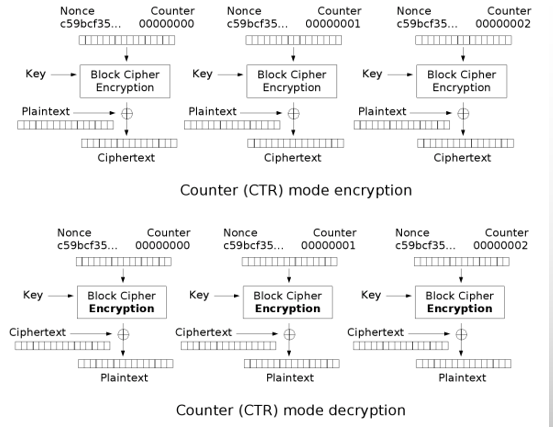
\includegraphics[height=3in]{./images/CTR.png}
% \caption{Diagrama CTR Cifrado}
% \label{fig:1-3-1}
%\end{subfigure}
%\end{figure}

%\pagebreak

%==================================================================================================================================================================


\section{Cómputo Nube. }
El cómputo nube definido así por el NIST, es un modelo para permitir un acceso a la red ubicuo, es decir, que se encuentra presente en todas partes al mismo tiempo y conveniente a un conjunto de recursos informáticos configurables (por ejemplo, redes, servidores, almacenamiento, aplicaciones y servicios) que se puede aprovisionar y liberar rápidamente con un esfuerzo mínimo de gestión o una interacción entre el proveedor de servicios.
Este modelo de cómputo nube se compone de 5 características esenciales, 3 modelos de servicio y 4 modelos de despliegue. \\ \\ 


\textbf{Características: }
\begin{itemize}
\item \textbf {Auto-servicio bajo demanda. } \\ Un consumidor puede proporcionar unilateralmente capacidades del tiempo del servidor y el almacenamiento en red, según se necesite automáticamente sin interacción con cada proveedor de servicios.
\item \textbf {Amplio acceso a la red. } \\ Las capacidades están disponibles a través de la red y se accede a través de mecanismos que promueven el uso por plataformas de clienteheterogéneas finas o gruesas (por ejemplo, teléfonos móviles, tablets, computadoras portátiles y estaciones de trabajo)
\item \textbf {Agrupación de recursos. } \\ Los recursos informáticos del proveedor se agrupan para servir a múltiples consumidores utilizando un modelo de múlti- usuario, con diferentes recursos físicos y virtuales asignados dinámicamente y reasignados de acuerdo con la demanda del consumidor. Hay una sensación de independencia de ubicación en que el cliente generalmente no tiene control o conocimiento sobre la ubicación exacta de los recursos proporcionados, pero puede especificar la ubicación en un nivel superior de abstracción (por ejemplo, país, estado o centro de datos). Ejemplos de recursos incluyen almacenamiento, procesamiento, memoria y ancho de banda de la red.
\item \textbf{Elasticidad rápida. } \\ Las capacidades pueden ser suministradas elásticamente y liberadas, en algunos casos de forma automática, para escalar rápidamente hacia fuera y hacia adentro proporcional a la demanda. Para el consumidor, las capacidades disponibles para la provisión a menudo parecen ser ilimitadas y pueden ser apropiadas en cualquier cantidad en cualquier momento.
\item \textbf{Servicio medido. } \\ Los sistemas de cómputo nube controlan y optimizan automáticamente el uso de recursos aprovechando una capacidad de medición en algún nivel de abstracción apropiado al tipo de servicio (por ejemplo, almacenamiento, procesamiento, ancho de banda y cuentas de usuario activas). El uso de recursos puede ser monitoreado, controlado y reportado, proporcionando transparencia tanto para el proveedor como para el consumidor del servicio utilizado.
\end{itemize} 


\textbf{Modelos de servicio. }
Entre los diversos tipos de servicios de cómputo en la nube proporcionados internamente o por proveedores de servicios de terceros, los más habituales son:
\begin{itemize}
\item \textbf {Software como Servicio (SaaS). } \\ La capacidad proporcionada al consumidor es utilizar las aplicaciones del proveedor que se ejecutan en una infraestructura en la nube. Las aplicaciones son accesibles desde varios dispositivos cliente a través de una interfaz de cliente ligero, como un navegador web (por ejemplo, correo electrónico basado en web) o una interfaz de programa. El consumidor no gestiona ni controla la infraestructura oculta de la nube, incluyendo la red, los servidores, los sistemas operativos, el almacenamiento o incluso las capacidades de las aplicaciones individuales, con la posible excepción de las limitadas configuraciones específicas de la configuración de la aplicación.
\item \textbf {Plataforma como Servicio (PaaS). } 
\item \textbf {Infraestructura como Servicio (IaaS). } 
\end{itemize} 


\textbf{Modelos de despliegue. }
\begin{itemize}
\item \textbf {Nube privada. } \\ La infraestructura de la nube está preparada para el uso exclusivo de una sola organización que comprende varios consumidores (por ejemplo, unidades de negocio). Puede ser propiedad, administrado y operado por el órgano.
\item \textbf{Nube de la comunidad. } \\ La infraestructura de la nube está preparada para uso exclusivo por una comunidad específica de consumidores de organizaciones que tienen preocupaciones compartidas (por ejemplo, misión, requisitos de seguridad, política y consideraciones de cumplimiento). Puede ser propiedad, administrado y operado por una o más de las organizaciones de la comunidad, un tercero, o una combinación de ellos, y puede existir dentro o fuera de las instalaciones.
\item \textbf{Nube pública. } \\ La infraestructura de la nube está preparada para el uso abierto por el público en general. Puede ser propiedad, administrado y operado por una organización comercial, académica u gubernamental, o alguna combinación de ellos. Existe en las instalaciones del proveedor de la nube.
\item \textbf{Nube híbrida. } \\ La infraestructura de la nube es una composición de dos o más infraestructuras de nube distintas (privadas, comunitarias o públicas) que siguen siendo entidades únicas, pero están unidas por una tecnología estandarizada o propietaria que permite la portabilidad de datos y aplicaciones (por ejemplo, burbujas de nube para equilibrar la carga entre Nubes).
\end{itemize} 




\textbf{Problemas en Cómputo Nube. }

\begin{itemize}
%\item \textbf {Abuso y mal uso del Cómputo Nube. } \\ Esta amenaza afecta principalmente a los modelos de servicio IaaS y PaaS y se relaciona con un registro de acceso a estas infraestructuras/plataformas poco restrictivo. Es decir, cualquiera con una tarjeta de crédito válida puede acceder al servicio, con la consecuente proliferación de spammers, creadores de código malicioso y otros criminales que utilizan la nube como centro de operaciones. 
\item \textbf {Interfaces y API poco seguros. } \\ Generalmente los proveedores de servicios en la nube ofrecen una serie de interfaces y API (del inglés, Application Programming Interface) para controlar e interactuar con los recursos. De este modo, toda la organización, el control, la provisión y la monitorización de los servicios cloud se realiza a través de estos API o interfaces. 
Dado que todo (autenticación, acceso, cifrado de datos, etc.) se realiza a través de estas herramientas, se hace necesario que los interfaces estén diseñados de forma segura, evitando así los problemas de seguridad, tanto los que son intencionados como los que se producen de forma accidental. 
%\item \textbf {Amenaza Interna. } \\ Como en todos los sistemas de información, la amenaza que suponen los propios usuarios es una de las más importantes, dado que tienen acceso de forma natural a los datos y aplicaciones de la empresa. En un entorno cloud esto no es en absoluto diferente ya que se pueden desencadenar igualmente incidentes de seguridad provocados por empleados descontentos y accidentes por error o desconocimiento. 
%Además, en muchos casos, es el propio proveedor del servicio el que gestiona las altas y bajas de los usuarios, produciéndose brechas de seguridad cuando el consumidor del servicio no informa al proveedor de las bajas de personal en la empresa. 
%Como es lógico, estos incidentes repercuten de forma importante en la imagen de la empresa y en los activos que son gestionados. 
%Los proveedores de servicio deberán proveer a los consumidores del servicio de medios y métodos para el control de las amenazas internas.
%\item \textbf {Problemas derivados de la tecnología compartida. } \\ Esta amenaza afecta a los modelos IaaS, ya que en un modelo de Infraestructura como Servicio los componentes físicos (CPU, GPU, etc.) no fueron diseñados específicamente para una arquitectura de aplicaciones compartidas. Se han dado casos en los que los hipervisores de virtualización podían acceder a los recursos físicos del anfitrión provocando, de esta forma, incidentes de seguridad. 
%Para evitar este tipo de incidentes se recomienda implementar una defensa en profundidad con especial atención a los recursos de computación, almacenamiento y red. Además, se ha de generar una buena estrategia de seguridad que gestione correctamente los recursos para que las actividades de un usuario no puedan interferir en las del resto. 
\item \textbf {Pérdida o fuga de información. } \\ Existen muchas formas en las que los datos se pueden ver comprometidos. Por ejemplo, el borrado o modificación de datos sin tener una copia de seguridad de los originales, supone una pérdida de datos. 
En la nube, aumenta el riesgo de que los datos se vean comprometidos ya que el número de interacciones entre ellos se multiplica debido a la propia arquitectura de la misma. Esto deriva en pérdida de imagen de la compañía, daños económicos y, si se trata de fugas, problemas legales, infracciones de normas, etc.
\item \textbf {Secuestro de sesión o servicio. } \\ En un entorno en la nube, si un atacante obtiene las credenciales de un usuario del entorno puede acceder a actividades y transacciones, manipular datos, devolver información falsificada o redirigir a los clientes a sitios maliciosos.
%\item \textbf {Riesgos por desconocimiento. } \\ Uno de los pilares de las infraestructuras cloud es reducir la cantidad de software y hardware que tienen que adquirir y mantener las compañías, para así poder centrarse en el negocio. Esto, si bien repercute en ahorros de costes tanto económicos como operacionales, no puede ser motivo para el deterioro de la seguridad por falta de conocimiento de esta infraestructura. 
%Para asistir en la toma de decisiones sobre las medidas de seguridad que se han de implantar en un entorno cloud es conveniente conocer, al menos en parte, la información técnica de la plataforma. Datos como con quién se comparte la infraestructura o los intentos de acceso no autorizados pueden resultar muy importantes a la hora de decidir la estrategia de seguridad. 
%La carencia de información de este tipo puede derivar en brechas de seguridad desconocidas por el afectado. 
\end{itemize} 


%Las funciones hash son usadas para construir una pequeña huella digital de la informaci\'on, si la informaci\'on es alterada tambi\'en la huella digital es alterada. Esta caracter\'istica hace que las funciones hash sean ampliamente usadas para verificar la integridad de datos.\\
%De manera formal, un funci\'on Hash es una Cuadrupla$(X,Y,K,H)$ donde:
%\begin{enumerate}
% \item $X$ es un conjunto de posibles mensajes.
% \item $Y$ es un conjunto finito de posibles resúmenes de mensajes o etiquetas de autenticación.
% \item $K$, el espacio de claves, es un conjunto finito de posibles claves.
% \item Para cada $k\quad \epsilon\quad K$, existe una función hash $h_k\quad \epsilon\quad H$. Parac ada $h_k: X \longrightarrow Y$.
% \cite{stinson}
%\end{enumerate}


%==================================================================================================================================================================







